\section{Attacco Denial of Service}
L'attacco di tipo \textit{Denial of Service} (DOS) consiste nel rendere non disponibili servizi offerti da computer o altri
dispositivi \cite{dos-definition}. Questo avviene esasperando di richieste la macchina o infrastruttura che viene scelta come
vittima.

\subsection{Vulnerabilità nelle reti cellulari}
Le reti cellulari non sono esenti da questo tipo di attacchi, anzi, sono una delle tipologie più frequenti e sopratutto difficile da risolvere
poichè le vulnerabilità che sfruttano sono organiche nell'architettura della rete.
Sono diversi i componenti che possono essere vulnerabili a un attacco DOS in una rete cellulare, gli obiettivi identificati come ottimi sono quelli
che comportano un maggior utilizzo delle risorse della rete.\\
Nelle prossime sezioni verranno illustrate le principali metodologie per fare un attacco di tipo \textit{Denial of Service} alle reti cellulari\cite{4g-dos-recap}.

\subsubsection{Radio Jamming}
Il \textit{Radio Jamming} è una tipologia di attacco \textit{Denial of Service} che consiste nel disturbare il segnale cellulare emettendo delle onde radio.
La realizzazione di questo tipo di attacco è molto semplice, basta procurarsi un trasmettitore che invia segnali ad alta energia nella banda cellulare di riferimento.\\
Un miglioramento del classico \textit{radio jamming} è lo \textit{smart jamming} che consiste nel saturare uno o più canali di comunicazione della rete. Questo fa sembrare 
il \textit{network} non disponibile a tutti gli utenti collegati a quella determinata cella.
\begin{figure}[h]
    \centering
    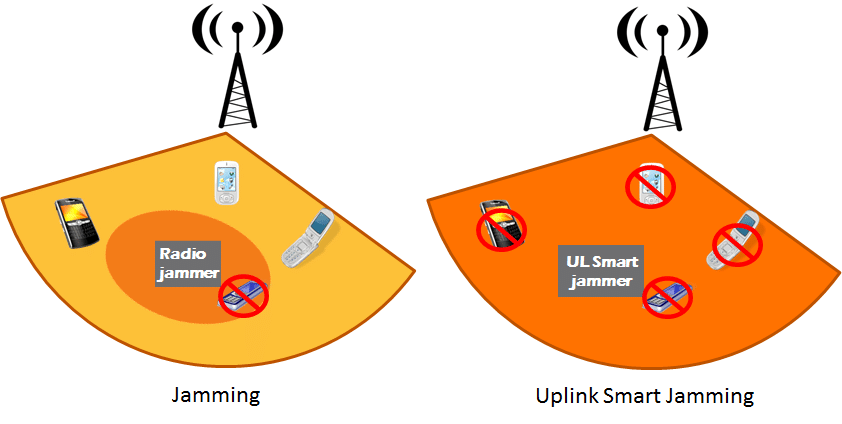
\includegraphics[width=0.7\textwidth]{images/dos-jamming.png}
    \caption{\textit{radio} e \textit{smart jamming}\cite{4g-dos-recap}}
\end{figure}\\

\subsubsection{Vulnerabilità di sistema}
Un altro classico modo per creare un interruzione di sistema in una rete cellulare è sfruttando le classiche vulnerabilità che si presentano spesso in qualsiasi tipo di computer.
Questo ovviamente perchè tutta l'architettura di una rete cellulare non è altro che \textit{server} con specifiche particolari.

\clearpage

\subsubsection{Botnet}
Questa è sicuramente una delle tipologie più diffuse, ed è il classico esempio di \textit{Distributed Denial Of Service}. L'attaccante, in questo caso, dispone del controllo di 
un grande numero di dispositivi infettati da \textit{malware} che possono essere attivati da lui per esasperare di richieste un determinato servizio.
\begin{figure}[h]
    \centering
    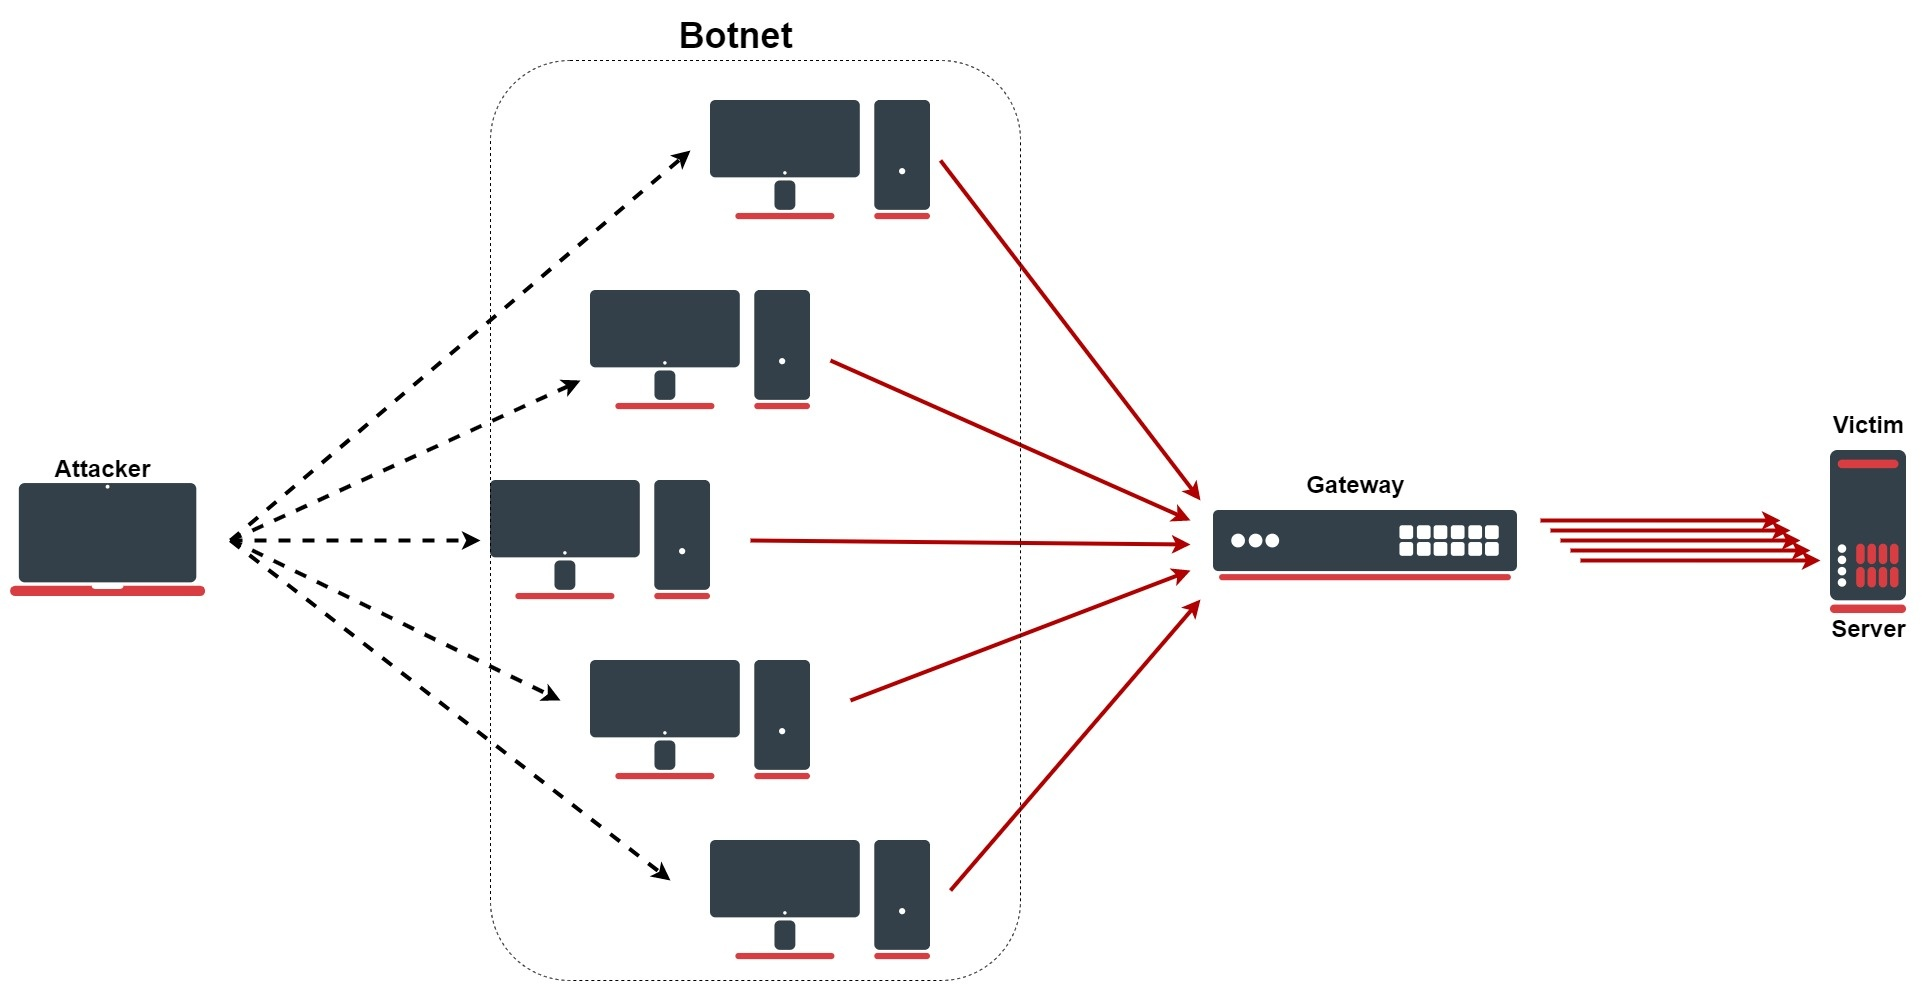
\includegraphics[width=0.5\textwidth]{images/ddos.jpg}
    \caption{Distributed Denial of Service}
\end{figure}\\

\subsubsection{Autenticazione}
Questo è uno dei più pericolosi poichè molto difficile da risolvere dato che è intrinseca nella architettura del sistema.
E' la tipologia di vulnerabilità che è stata scelta per confrontare la sicurezza della architettura 5G con quelle precedenti.
Il suo funzionamento si basa sull'esasperare di richieste di autenticazione i sistemi identificativi delle reti cellulari, che solitamente 
sono i componenti con più traffico della rete. Per esempio, nelle generazioni 2G e 3G, è la HLR che viene identificata come componente critico del
sistema.\\
Questa vulnerabilità si trova nel meccanismo di autenticazione dei dispositivi denominato \textit{Authentication and Key Agreement} (AKA) dove un dispositivo
non autenticato forza delle computazioni all'interno del \textit{Core Network} che consumano più risorse della richiesta stessa\cite{umts-dos}.
Ad aumentare la pericolosità di questa vulnerabilità è la possibilità di creare computazioni nel \textit{Core Network} senza essere effettivamente autenticati, e quindi 
senza disporre di una SIM valida. Questa tipologia di attacchi, definiti come SIM-less, verranno presi come riferimento per sfruttare questa vulnerabilità come illustrato per le 
reti GSM\cite{gsm-dos-simless} e UMTS\cite{umts-dos}.

\clearpage

\subsection{Misurazione}
Per capire quale componente della rete sia il più vulnerabile a un attacco DOS si devono fare delle misurazioni sui vari componenti del \textit{network}.
In questo modo è possibile capire in quale punto si possono creare dei rallentamenti o \textit{bottleneck} dovuti a un sovraffollamento di richieste.\\
In \cite{measuring-dos} vi è una dettagliata spiegazione di come procedere con queste misurazioni e sopratutto come quantificare il numero di dispositivi che 
servono all'attaccante per completare l'attacco con successo.

\begin{figure}[h]
    \centering
    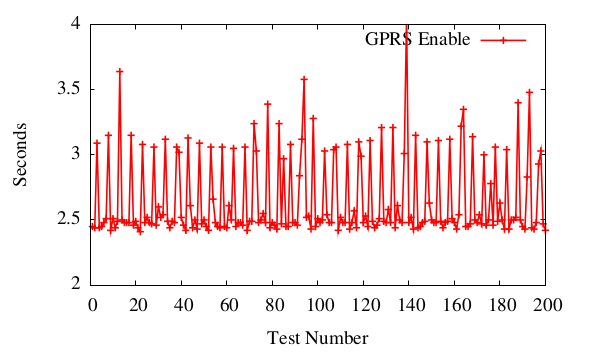
\includegraphics[width=0.7\textwidth]{images/hlr-measuring.png}
    \caption{Misurazione tempi di risposta HLR con \textit{location updates}\cite{measuring-dos}}
\end{figure}